\chapter{Data Exploration}
\label{chapter:data}
\section{EU-Forest Dataset}

EU-Forest is a dataset containing tree species and genera for nearly
$250,000$ plots across Europe \cite{eu_forest_data}. Each plot is 1\,km\,×\,1\,km
and may contain multiple tree species and genera.

\begin{figure}[!htb]
    \centering
    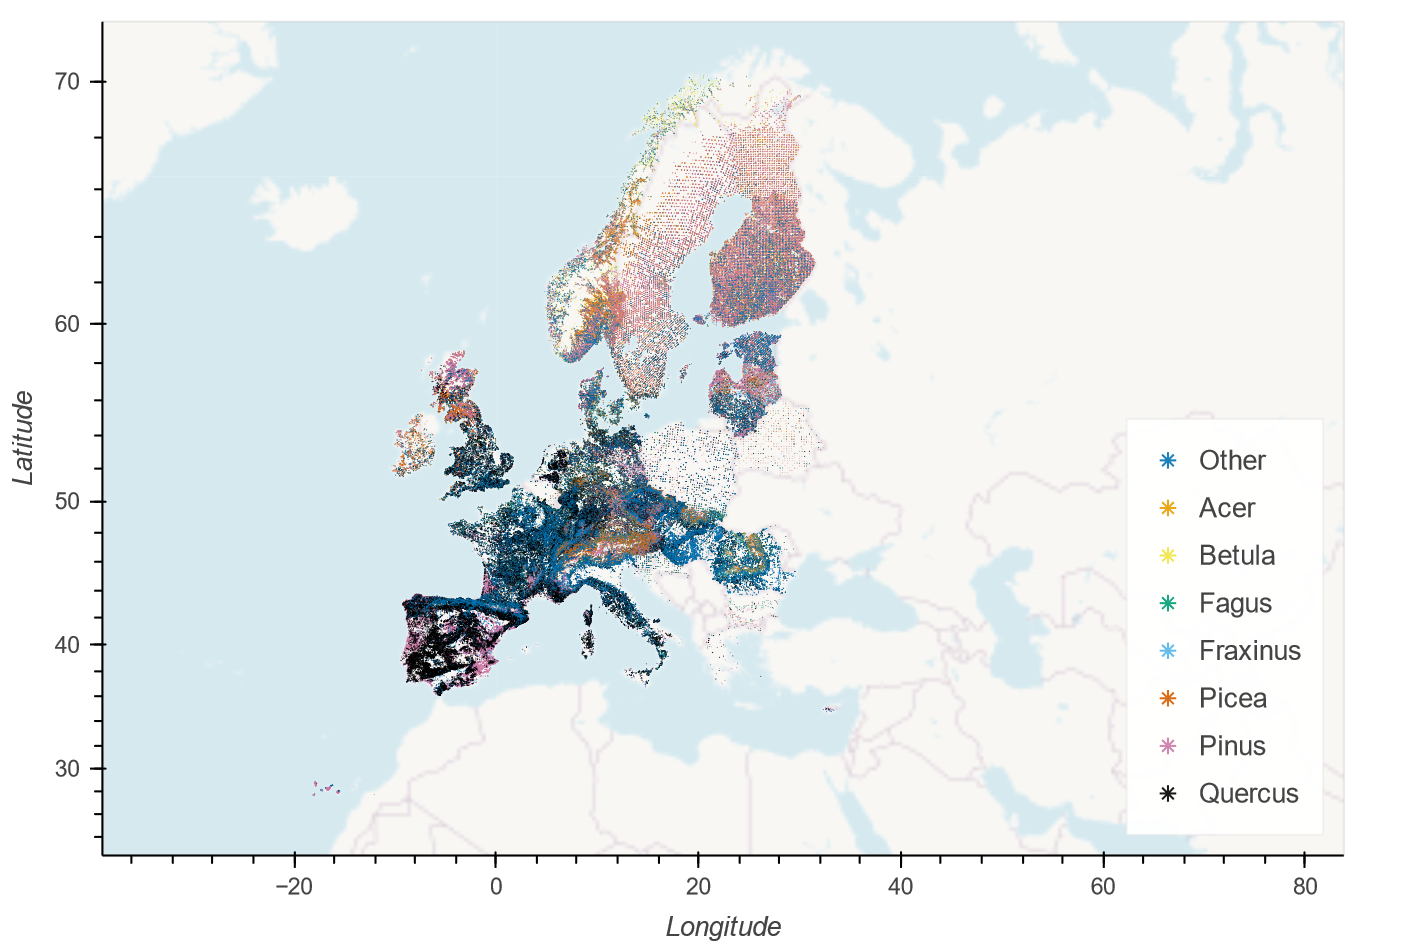
\includegraphics[width=0.9\linewidth]{figures_labels/genus_cutoff_map.png}
    \caption{Map of the most common tree genera in EU-Forest.}
    \label{fig:genus_cutoff_map}
\end{figure}

Fig.\,\ref{fig:genus_cutoff_map} shows the distribution of tree genera in the EU-Forest dataset
across 21 European countries. In this figure, the label 'Other' is an umbrella class for 70 
tree genera.

\begin{figure}[!htb]
    \centering

    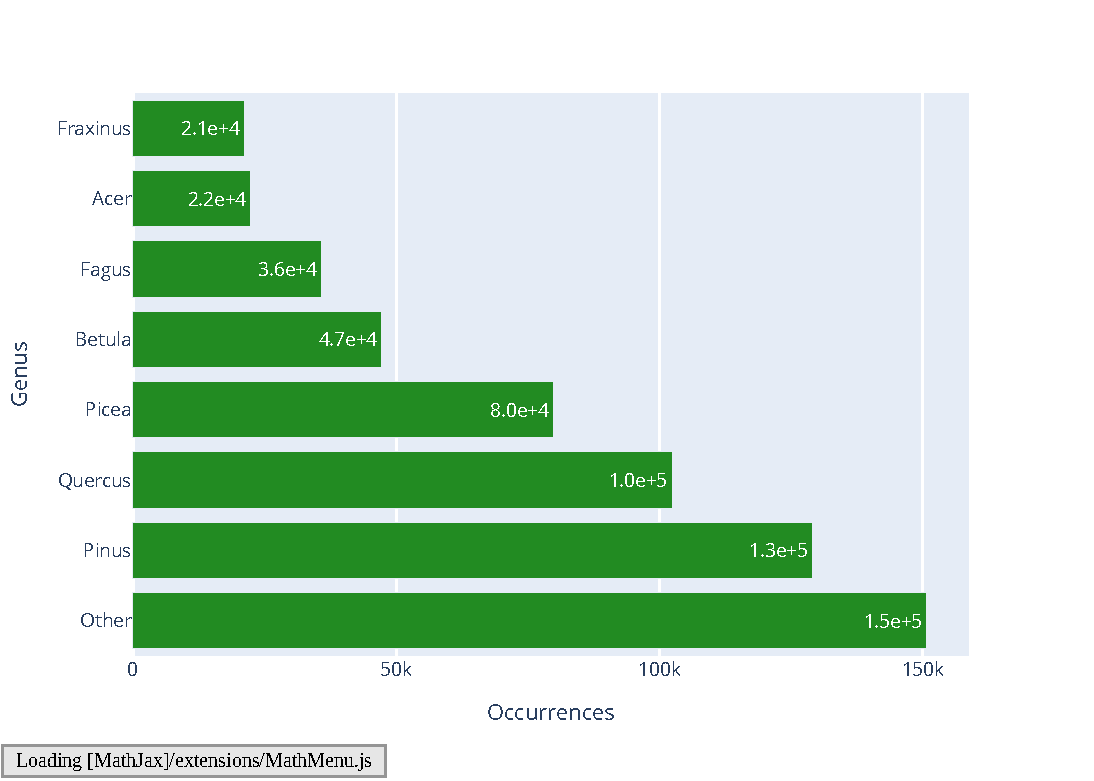
\includegraphics[width=0.48\linewidth, trim={0 0 2cm 0}]{figures_labels/genus_cutoff.pdf}
    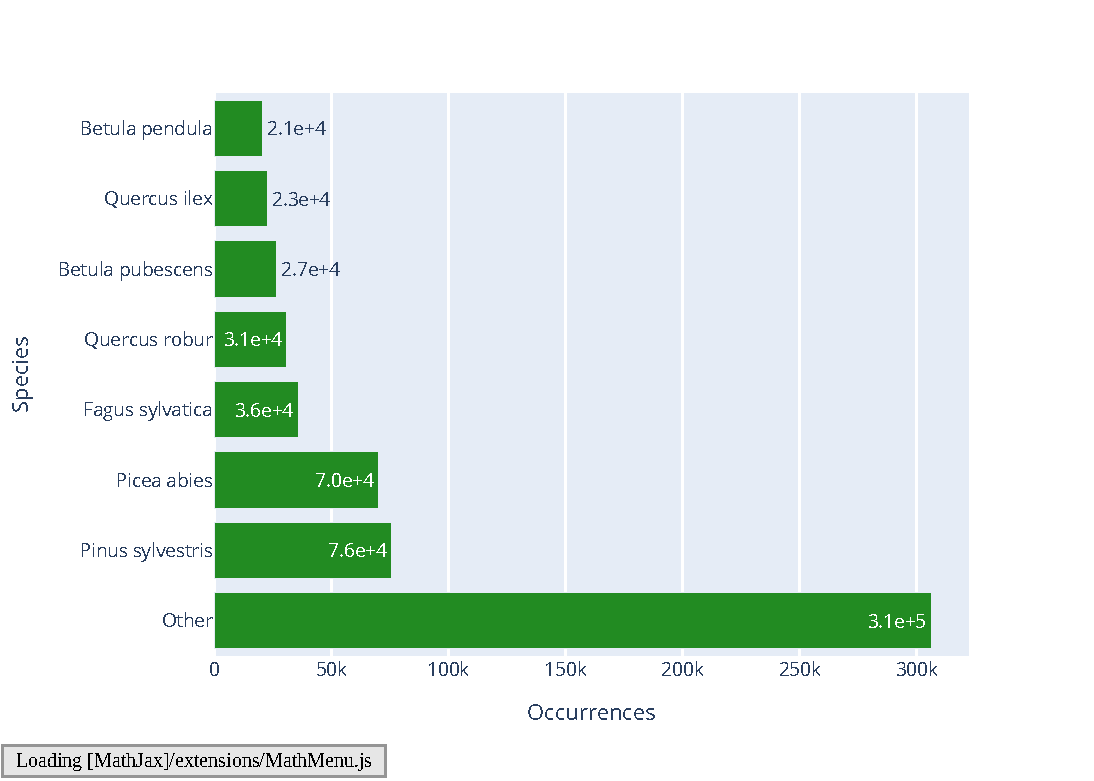
\includegraphics[width=0.48\linewidth, trim={0 0 2cm 0}]{figures_labels/species_cutoff.pdf}

    \caption{Distribution of genera (left) and species (right) in EU-Forest.}
    \label{fig:cutoff_barplots}
\end{figure}

In Fig.\,\ref{fig:cutoff_barplots}, both plots show a class imbalance. 
Classes with occurrences below 20\,k were grouped and labeled as 'Other'.

\begin{figure}[!htb]
    \centering

    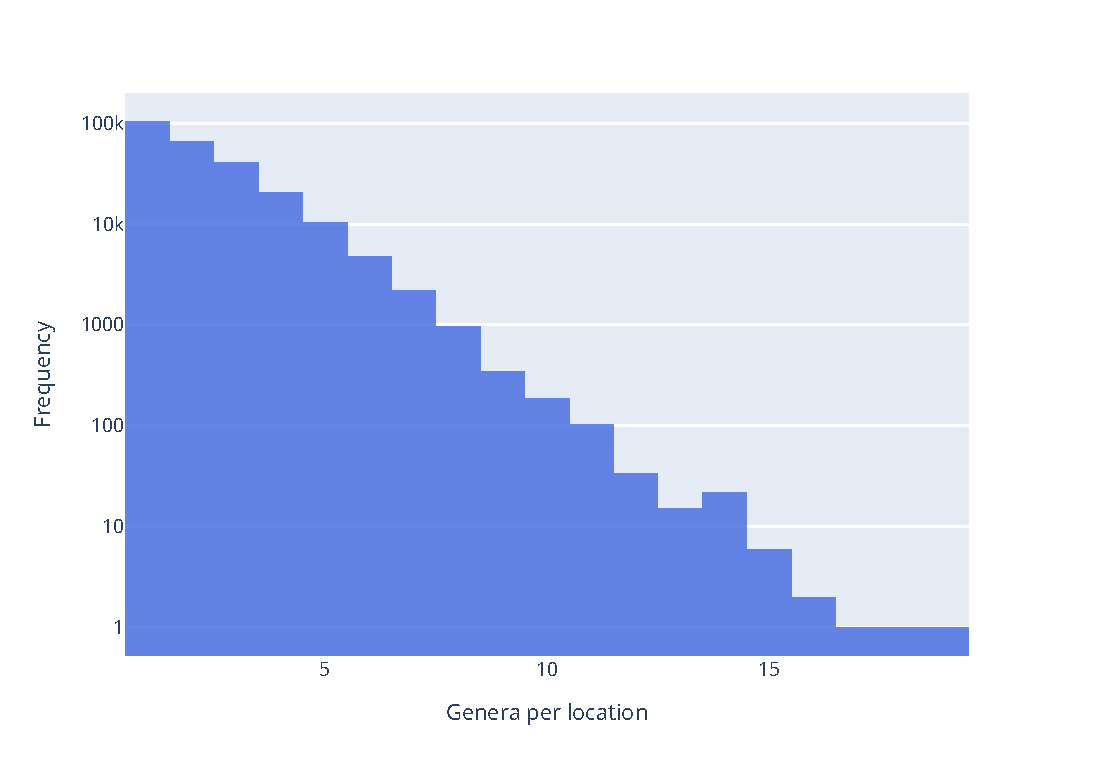
\includegraphics[width=0.48\linewidth, trim={0 0 2cm 0}]{figures_labels/grouped_genus.pdf}%
    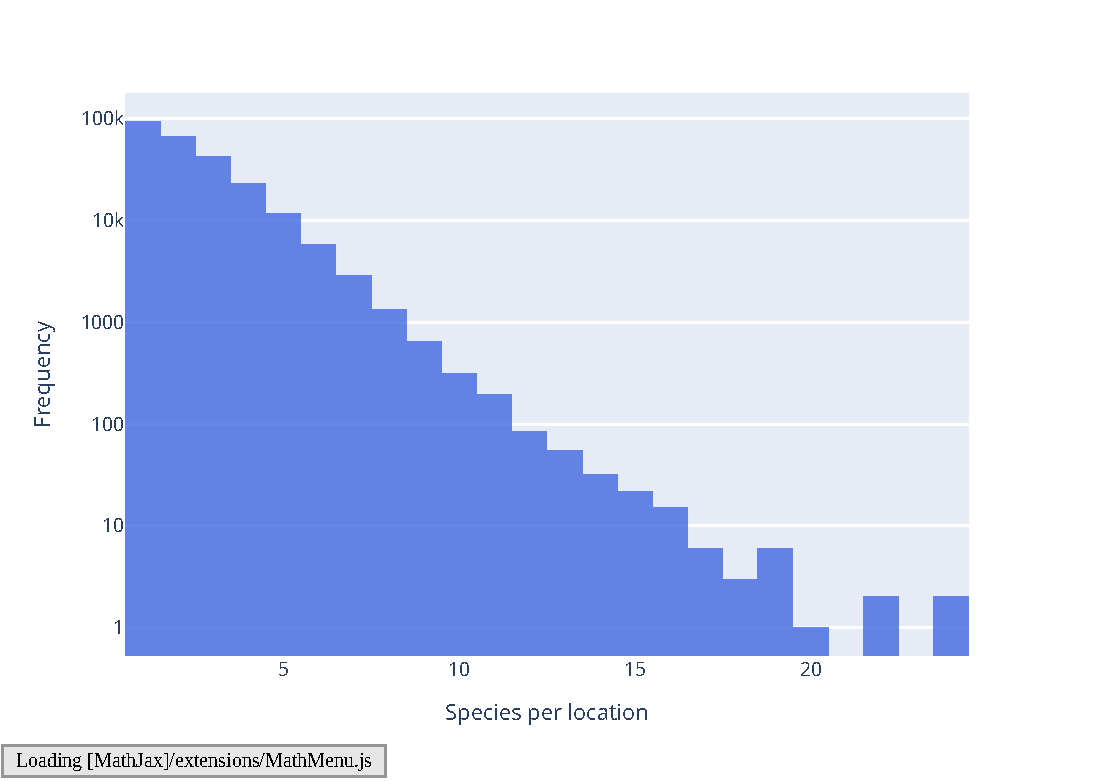
\includegraphics[width=0.48\linewidth, trim={0 0 2cm 0}]{figures_labels/grouped_species.pdf}

    \caption{Distribution of genera (left) and species (right) per location.}
    \label{fig:grouped_histograms}
\end{figure}

\section{Sentinel-2}

\begin{figure}[!htb]
    \centering

    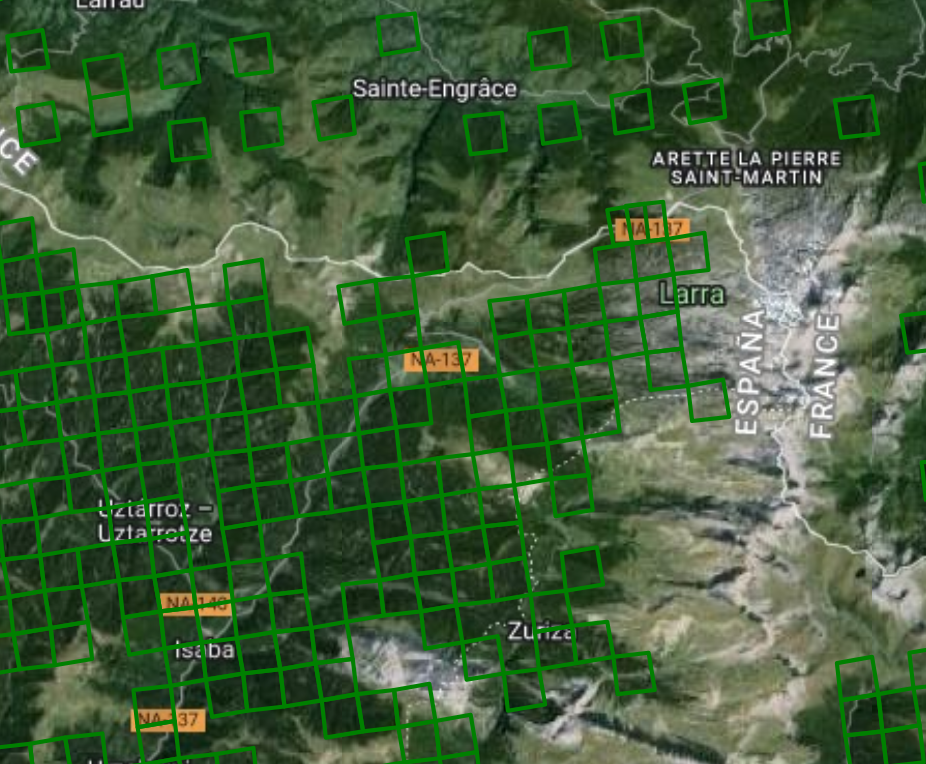
\includegraphics[width=0.48\linewidth]{figures_labels/sample_area_earth.png}
    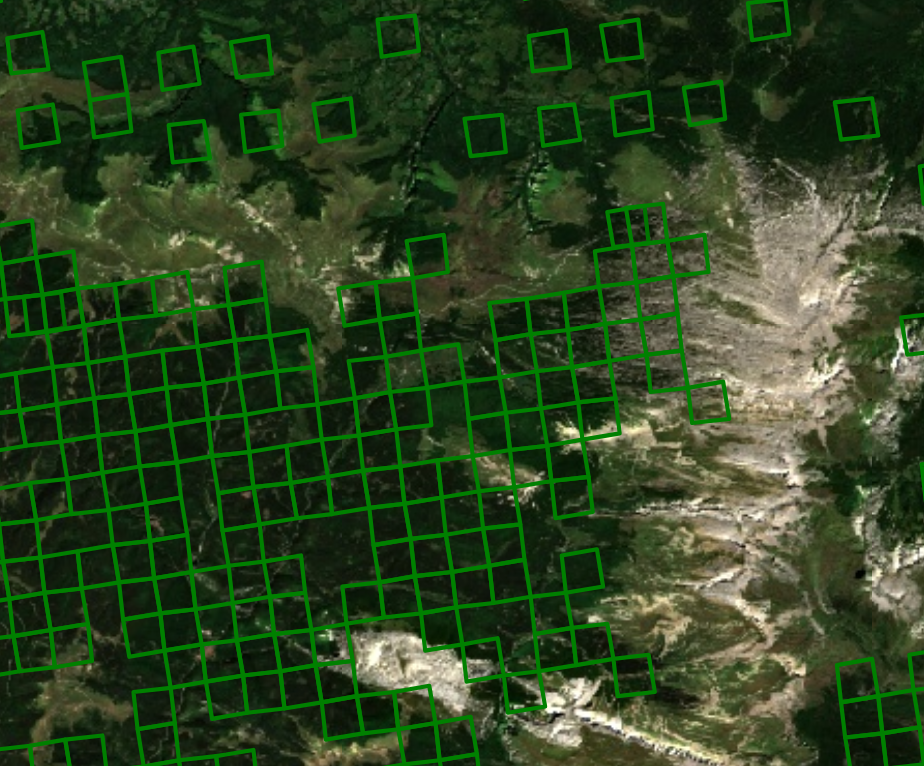
\includegraphics[width=0.48\linewidth]{figures_labels/sample_area_sentinel.png}

    \caption{Sample locations overlayed on Google Earth (left) and Sentinel-2 (right).}
    \label{fig:_label_sample_area}
\end{figure}

\begin{figure}[!htb]
    \centering

    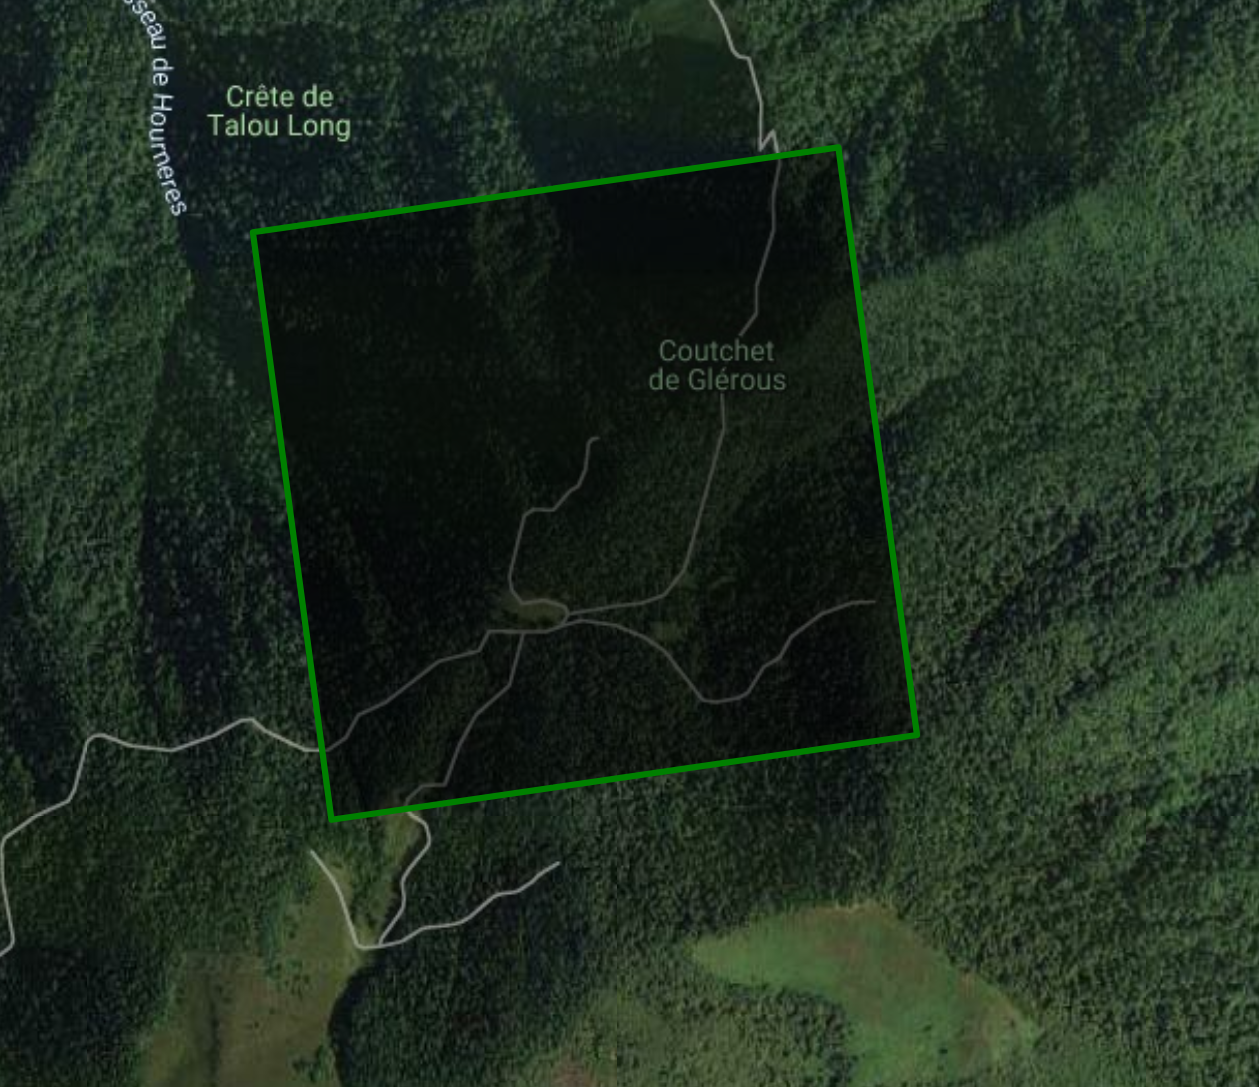
\includegraphics[width=0.48\linewidth]{figures_labels/sample_earth.png}
    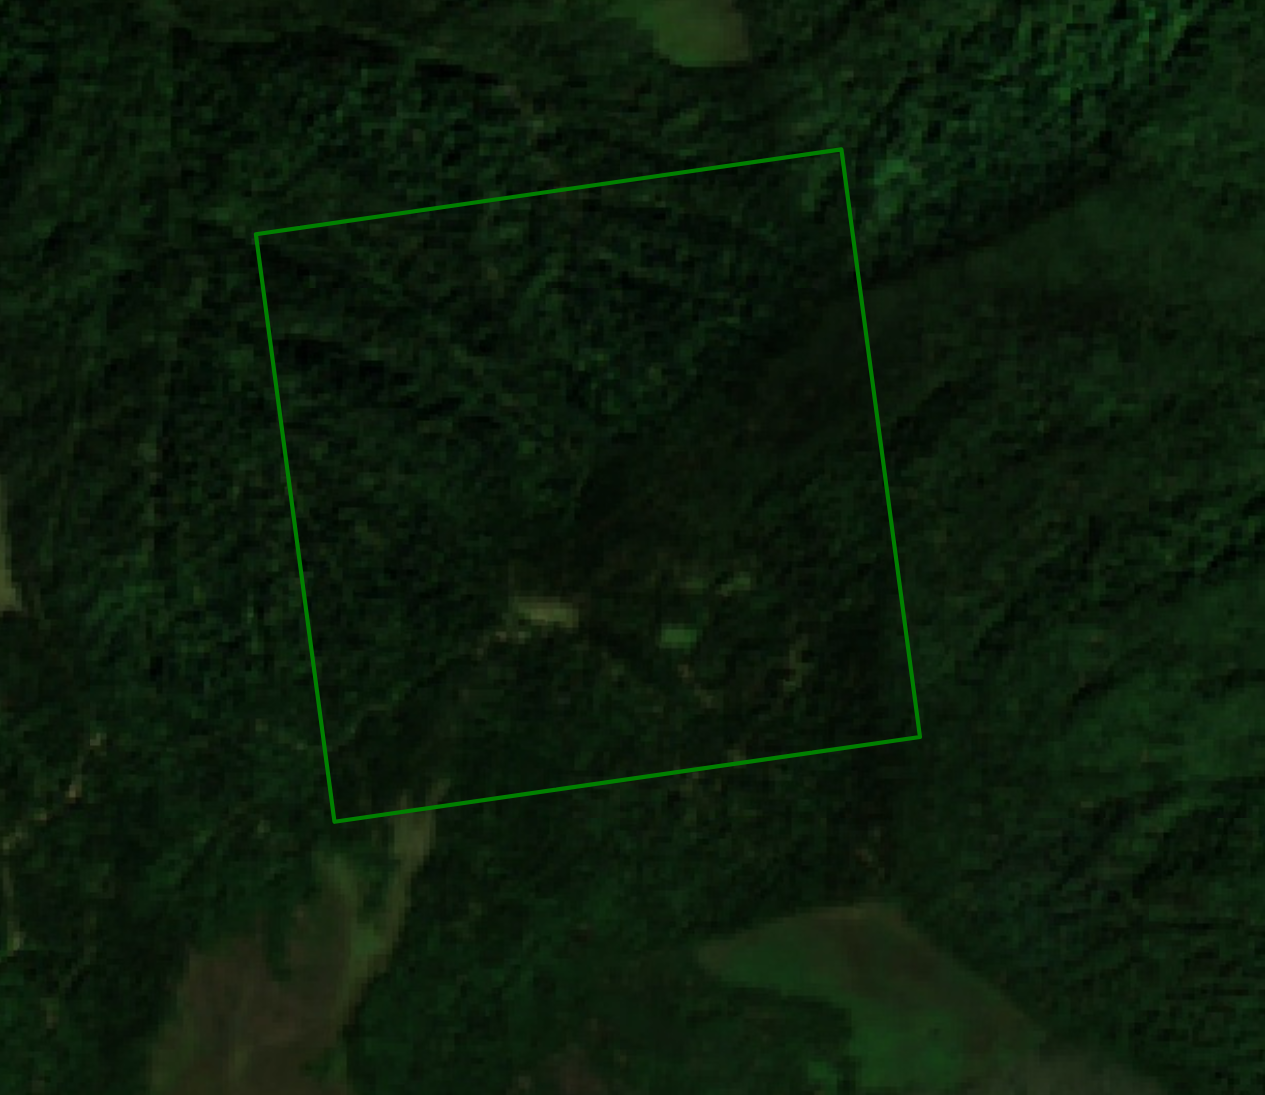
\includegraphics[width=0.48\linewidth]{figures_labels/sample_sentinel.png}

    \caption{Sample locations overlayed on Google Earth (left) and Sentinel-2 (right).}
    \label{fig:label_sample}
\end{figure}